\documentclass[11pt]{article}
\usepackage[margin=1in]{geometry}
\usepackage{amsmath,amssymb}
\usepackage{graphicx}
\usepackage{booktabs}
\usepackage[colorlinks=true,linkcolor=blue,citecolor=blue,urlcolor=blue]{hyperref}

% --- the only two lines to edit before submission ---
\newcommand{\authorname}{Singularity}
\newcommand{\affiliation}{}

\title{Crystal structure versus composition for the formation energy\\ of unseen perovskite formulas}
\author{\authorname\\ \small \affiliation}
\date{\today}

\begin{document}
\maketitle

\begin{abstract}
Composition-only models are a common first screen for new ceramic materials. We measure how much a small crystal
graph neural network gains over them when the formulas to be predicted are entirely absent from training. On the
Matbench perovskites benchmark (18,928 structures, DFT formation energy), with all structures of a reduced formula kept
in one partition, the graph network reached a mean test error of 0.059 and 0.055 eV per unit cell in two
independent splits, against 0.403 and 0.419 for LightGBM on elemental fractions and 0.437 and 0.451 for ridge
regression. The graph network explained 98.7--98.8\% of the variance, LightGBM 47--49\%. Paired bootstrap intervals
over 1,930 held-out formula groups put the reduction against LightGBM at 0.341 to 0.368 and 0.359 to 0.388 eV.
A deliberately small network, trained in about five minutes per seed on a CPU, is enough to obtain this gap.
\end{abstract}

\section{Introduction}
Perovskite oxides and related compounds are a central family of functional ceramics. Screening models often use
composition alone, because the crystal structure of a hypothetical compound is not always known. Graph neural
networks that read the crystal structure~\cite{cgcnn} are known to predict DFT energies well on random splits of
benchmarks such as Matbench~\cite{matbench}. Here we ask a narrower, practical question: when the reduced formula itself
is new, how large is the advantage of structure over composition, measured on the same splits, with simple and
reproducible models?

\section{Methods}
\paragraph{Data.} Matbench perovskites~\cite{matbench}, adapted from the calculations of Castelli et
al.~\cite{castelli}: 18,928 crystal structures with 9,646 reduced formulas; target
\emph{e\_form}, the DFT formation energy in eV per unit cell.
\paragraph{Splits.} Grouped by reduced formula, so that all structures of a formula are in one partition. Split 1
(seeds 2026/2027): 13,242 training, 1,898 validation and 3,788 test structures; split 2 (seeds 2028/2029): 13,264,
1,893 and 3,771. Zero formula overlap between partitions was verified in both splits.
\paragraph{Models.} Crystal graph network: learned atomic-number embeddings, edges to up to 16 nearest periodic
neighbours within 8~\AA, 16 radial-basis distance features, three mean-aggregating message-passing updates and mean
pooling; AdamW on a standardised target with early stopping on validation error, three seeds per split.
Composition baselines on the 118-dimensional elemental-fraction vector: ridge regression ($\alpha=10$) and LightGBM
(700 trees, learning rate 0.04, 31 leaves). All settings and both splits were fixed before the runs; the test sets
were used only for final scoring.
\paragraph{Comparison.} Mean absolute error (MAE), root mean squared error and $R^2$; for the main contrast, the
average of the three network seeds against LightGBM, with a paired bootstrap over held-out formula groups (2,000
replicates).

\section{Results}
\begin{table}[h]
\centering
\begin{tabular}{lrrrrrr}
\toprule
 & \multicolumn{3}{c}{split 1} & \multicolumn{3}{c}{split 2} \\
model & MAE & RMSE & $R^2$ & MAE & RMSE & $R^2$ \\
\midrule
crystal graph network & \textbf{0.0586} & 0.0852 & 0.987 & \textbf{0.0554} & 0.0825 & 0.988 \\
LightGBM, composition & 0.4031 & 0.5352 & 0.485 & 0.4189 & 0.5524 & 0.473 \\
ridge, composition & 0.4367 & 0.5724 & 0.412 & 0.4507 & 0.5863 & 0.406 \\
\bottomrule
\end{tabular}
\caption{Test results for unseen formulas, in eV per unit cell. Network: mean of three seeds (standard deviation of
MAE 0.0045 and 0.0026).}
\label{tab:results}
\end{table}

\begin{figure}[h]
\centering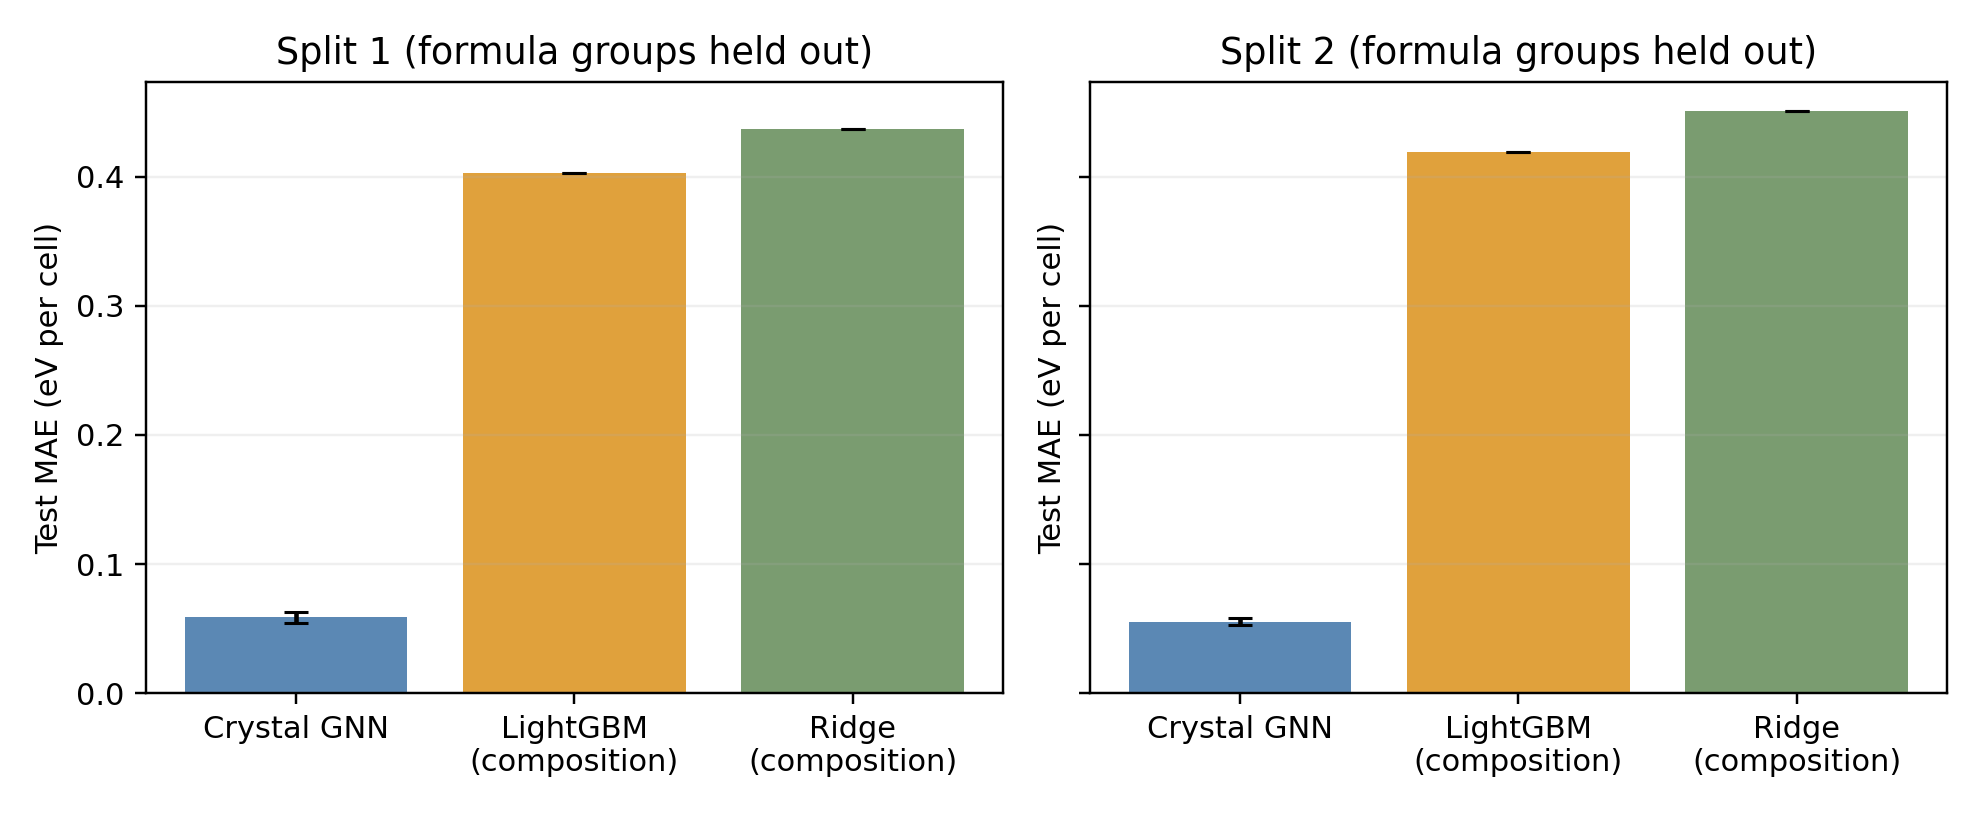
\includegraphics[width=.9\linewidth]{fig_results.png}
\caption{Test MAE on two held-out sets of formula groups. Error bars: standard deviation over the three network
seeds; the composition baselines are single fits.}
\label{fig:results}
\end{figure}

\begin{itemize}
\item \textbf{Large and reproducible gap.} The seed-averaged network reduced MAE against LightGBM by 0.355~eV in split
1 (interval 0.341 to 0.368) and by 0.373~eV in split 2 (0.359 to 0.388).
\item \textbf{Composition explains half the variance.} For new formulas, elemental fractions alone reach $R^2$ below
0.5; adding the crystal graph raises it to 0.99.
\item \textbf{Cost.} About five minutes per network seed on a CPU, against 0.3 seconds for LightGBM.
\end{itemize}

\section{Discussion}
For perovskite formation energies, knowing the arrangement of atoms is worth almost an order of magnitude in error
when the formula is new. This quantifies, on a strict formula-grouped protocol, a gap that random splits can hide:
on random folds the same formula with a different structure can appear in training. For screening hypothetical
compositions without a known structure, the composition-only error reported here is the realistic one.

For ceramic screening this suggests a direction worth testing: feeding even an approximate structure, for example a
prototype lattice, may pay off more than refining a composition-only model.

\paragraph{Limitations.} One computational dataset of one materials family, with DFT rather than measured energies.
Larger graph networks reported on Matbench reach lower errors; the aim here is the size of the gap, not the best
accuracy. The composition baselines use elemental fractions without engineered descriptors.

\paragraph{Reproducibility.} \texttt{experiment.py} runs both splits and the consolidation in order.
\texttt{results.json} contains the formula-overlap audit, per-seed metrics, the bootstrap and run times for both
splits; per-structure test predictions are in \texttt{code/}.

\paragraph{Origin of the question.} The question came from an automated forecast (Singularity v3, registered on 5
November 2026 with a SHA-256 fingerprint, view without generative AI) that graph neural networks would enter the subfield \emph{Ceramics and
Composites}. The forecast concerned the arrival of the method, not the result of this study.

\begin{thebibliography}{9}
\bibitem{matbench} A.~Dunn, Q.~Wang, A.~Ganose, D.~Dopp and A.~Jain, Benchmarking materials property prediction
methods: the Matbench test set and Automatminer reference algorithm, \emph{npj Computational Materials} 6, 138
(2020), doi:10.1038/s41524-020-00406-3.
\bibitem{castelli} I.~E.~Castelli et al., New cubic perovskites for one- and two-photon water splitting using the
computational screening approach, \emph{Energy \& Environmental Science} 5, 9034--9043 (2012).
\bibitem{cgcnn} T.~Xie and J.~C.~Grossman, Crystal graph convolutional neural networks for an accurate and
interpretable prediction of material properties, \emph{Physical Review Letters} 120, 145301 (2018).
\end{thebibliography}
\end{document}
